\chapter{Implementazione}
\label{chapter2}

Questo capitolo focalizzerà l'attenzione del lettore sull'implementazione \textit{\textbf{front-end}} adottata.
\\Con il termine front-end si intende la parte di un sistema software che gestisce l’interazione con l’utente o con sistemi esterni che producono dati di ingresso. Concerne tutte le parti visibili all’utente, con cui può interagire e generare dati che verrano trasmessi al back- end, dove verrano elaborati.
\\Il capitolo concernerà il Sistema Operativo scelto, l'ambiente di sviluppo, le API utilizzate e relativo utilizzo, la struttura generale dell'applicazione.
\\Successivamente si entrerà nel dettaglio di ogni singolo componente di cui è composta l'applicazione, discutendone ampiamente, sia dal punto di vista tecnico, sia per le scelte implemementative adottate.

\section{Sistema Operativo}

Il sistema operativo, su cui eseguire l'applicazione mobile, che si è deciso di utilizzare per questo progetto, è stato \textbf{Android}.
\\Android è un sistema operativo per dispositivi mobili sviluppato da Google e basato sul kernel Linux.
\\Ad aprile 2017, Android, è il sistema operativo per dispositivi mobili più diffuso al mondo, con una fetta di mercato attestatasi a quota 62,94\% sul totale, seguito da iOS con il 33,9\% \cite{developers2011android}.
\\L'applicazione realizzata, è un'applicazione nativa Android, ovvero creata esclusivamente per questo sistema operativo. La scelta è ricaduta su Android, poichè copre la maggior parte di mercato rispetto ad iOS.
\\Inoltre, un'app nativa, ha alcuni vantaggi rispetto ad un'app ibrida (ovvero un'applicazione rivolta a diversi sistemi operativi), fra cui: maggiore velocità e accesso più facile a tutte le funzionalità del telefono.
\\I linguaggi utilizzati per la realizzazione dell'app sono stati due: \textbf{Java} e \textbf{XML}.
\\Si è scelto Java poichè è risultato il linguaggio più idoneo, consono e diffuso per lo sviluppo di app di questo tipo.

\section{Ambiente di sviluppo}

L'ambiente che si è deciso di utilizzare per lo sviluppo e l'implementazione dell'applicazione è stato \textbf{Android Studio}.
\\Android Studio è un ambiente di sviluppo integrato (IDE) per lo sviluppo per la piattaforma Android. Si è scelta questa piattaforma poichè risulta la più stabile e compatibile, praticamente, con tutti i dispositivi Android e permette anche di emulare, in tempo reale, un dispositivo virtuale per provare e testare la propria applicazione.
\\Inoltre, Android Studio è un software molto diffuso quindi è stato relativamente facile trovare la documentazione e i tutorial per imparare ad utilizzarlo. In più, tra i vantaggi ci sono: il poter firmare le applicazioni, uno strumento per il disegno della UI, la possibilità di fare test per le performance e il controllo di versioni; tutto questo senza dover installare nessun plug-in.
\\Per testare e provare l'applicazione, è stato utilizzato un dispositivo fisico, ovvero un Samsung Galaxy S7 con Android 8.0, poichè è risultato più semplice, in fase di implementazione, provare le varie funzionalità dell'applicazione.

\section{API}
Un elemento fondamentale delle applicazioni sono le API.
\\Con il termine application programming interface (API) si indica un insieme di procedure atte al completamento di un dato compito \cite{api}. Spesso tale termine designa le librerie software di un linguaggio di programmazione. Una buona API fornisce una “scatola nera”, cioè un livello di astrazione che evita al programmatore di sapere come funzionano le API ad un livello più basso. Questo permette di riprogettare o migliorare le funzioni all’interno dell’API senza cambiare il codice che si affida ad essa.
\\Le API permettono di espandere le funzionalità di un programma. Per uno sviluppatore mettere a disposizione un set di API di un suo software significa dare la possibilità ad altri di interagire con la sua piattaforma e, soprattutto, estendere le funzioni e le caratteristiche della struttura base della piattaforma. In altri termini, le API sono un ottimo strumento per promuovere un programma offrendo ad altri un modo per interagirci.
\\Sono quindi degli strumenti di programmazione che vengono messi a disposizione degli sviluppatori dalle maggiori software house e industrie del mondo informatico come Microsoft, Google e Facebook. Servono principalmente per facilitare la realizzazione e per espandere le funzionalita` di applicazioni di vario genere. 
\\Le API possono assumere diverse “forme”: possono essere delle librerie di funzioni che permettono al programmatore di interagire con un programma o una piattaforma software o semplicemente una serie di “chiamate” a parti di un programma che uno sviluppatore può utilizzare per abbreviare il suo lavoro.

\subsection{Utilizzo delle API}
Utilizzando un’API, un programmatore può far interagire due programmi (o due piattaforme, o un programma e una piattaforma) altrimenti tra loro incompatibili. Si possono quindi estendere le funzionalita` di un programma ben oltre le reali intenzioni dello sviluppatore o della software house che l’ha realizzato. Un esempio pratico sono le API di Google Maps che sono a disposizione di tutti gli sviluppatori che le volessero utilizzare per un loro programma o piattaforma web. 
\\Sfruttando le API, ad esempio, è possibile utilizzare il servizio di cartografia digitale di Google per realizzare delle mappe personalizzate; oppure integrarle in siti web per servizi di ricerca georeferenziati; o ancora utilizzarle all’interno di applicazioni per smartphone e tablet.
\section{Struttura generale}

In questa sezione verrà presentata, la struttura generale dell'applicazione. La struttura dell'app è stata, di volta in volta, aggiornata e modificata durante l'implementazione del progetto, fino a presentarsi in questo modo.
\\L'applicazione si suddivide principalmente in 3 macro-aree:
\begin{itemize}
    \item Activity e classi \textit{.java}
    \item Risorse (Layout e values)
    \item AndroidManifest.xml
\end{itemize}
Le Activity e i rispettivi layout sono definiti nella tabella \ref{tabella}:

\begin{table}[h!]
\centering
    \begin{tabular}{||c c||} 
         \hline
         \textbf{ACTIVITY} & \textbf{LAYOUT} \\ [0.5ex] 
         \hline\hline
         MapsActivity.java & activity\_maps.xml \\ 
         MicrophoneActivity.java & activity\_microphone.xml  \\
         ModifyPhotoActivity.java & activity\_modify\_photo.xml \\
         ModifyVideoActivity.java & activity\_modify\_video.xml  \\
         ModifyVoiceNoteActivity.java & activity\_modify\_voice\_note.xml  \\ 
         PostActivity.java & activity\_post.xml \\
         TextNoteActivity.java & activity\_text\_note.xml \\ [1ex] 
         \hline
    \end{tabular}
    \caption {\textit{Activity e rispettivi layout}}
    \label{tabella}
\end{table}
\noindent
Inoltre, è stata utilizzata un'interfaccia \textit{\textbf{FileInformation.java}} e altre tre classi di appoggio \textit{\textbf{SavingOfFile.java}},  \textit{\textbf{MySingleton.java}} e \textit{\textbf{GenericFileProvider.java}}.
\\Nella sezione \ref{activity} verrà ampiamente discusso lo scopo di ogni Activity e classe Java implementata.
\\Nella sezione \ref{layout} verranno presentati i layout ma la loro presentazione verrà rimandata nel capitolo \ref{chapter3}.
\\Nella sezione \ref{values} verrà lasciato uno spazio per presentare le risorse utilizzate durante l'implementazione.
\\Nella sezione \ref{manifest} verrà presentato l'Android Manifest, la sua utilità e come è stato implementato.

\subsection{Activity e Classi Java}
\label{activity}
L’Activity è l’elemento principale di un’applicazione Android ed è essenzialmente una finestra che contiene l’interfaccia utente e può essere quindi vista come una schermata.\\
Il suo scopo è quello di consentire un’iterazione con l’utente. Un’applicazione può avere una o più Activity, ma solo una schermata alla volta può essere in primo piano. Vi è quindi un’Activity stack dove sono registrate tutte le Activity e si può passare da un’Activity all’altra grazie all’Activity Manager.\\
L'applicazione presenta \textbf{7 Activity} ognuna delle quali verrà ripresa poco più avanti dettagliatamente, spiegandone l'utilità.\\
Le Activity implementate sono le seguenti:
\begin{itemize}
\item MapsActivity.java
\item MicrophoneActivity.java
\item ModifyPhotoActivity.java
\item ModifyVideoActivity.java
\item ModifyVoiceNoteActivity.java
\item PostActivity.java
\item TextNoteActivity.java
\end{itemize}

\subsubsection{MapsActivity.java}
Questa è l'Activity che si incontra appena si apre l'applicazione, ovvero quella che rappresenta la mappa di Google Maps.
\\Si è deciso di iniziare da questa Activity, in questo modo, poichè si è pensato che era un ottimo modo di contestualizzare l'obiettivo dell'applicazione dando all'utente un feedback su dove si potesse trovare in un determinato ambiente ed orientarsi al suo interno.
\\La posizione del dispositivo viene continuamente aggiornata ogni qualvolta l'utente si sposti.


\subsubsection{PostActivity.java}
Questa è l'Activity principale dell'applicazione, ed è stata implementata inizialmente ispirandosi al \textit{"Aggiungi luogo"} di Google Maps, per poi riprogettarla unendo una vista basata su CardView e su due TextInputLayout poichè si è rivelata la miglior soluzione per quanto riguarda lo sviluppo di questo tipo di applicazione, più semplice ed intuitiva.
\\All'interno delle CardView sono stati implementati diverse componenti, come: le rispettive icone dei file multimediali, il numero dei file aggiunti fino a quel momento ed infine un bottone per la modifica dei file salvati in locale fino a quel punto. Foto e video verranno creati direttamente all'interno di questa Activity quando si apriranno rispettivamente fotocamera e videocamera.
\\L'invio dei file al database è stato eseguito sfruttando la libreria Volley, che si riprenderà in seguito nella sezione \ref{volley}, convertendo tutti i file acquisiti fino a quel momento in \textit{Base64}, in quanto si è visto che è il formato più diffuso per l'invio di file multimediali attraverso richieste \textit{POST} di tipo HTTP. 
\\Inoltre è stata implementata la creazione di un file di tipo \textit{CSV} che includesse le informazioni recuperate all'interno di questa Activity, come: latitudine, longitudine, nome del luogo ed indirizzo; così che si potesse, tramite espressioni regolari, recuperare un certo tipo di informazioni.
\\Al momento della stesura di questa relazione, non è stato ancora implementato l'invio al database di questo file, poichè, lato back-end, non è stato predisposta la ricezione di questo file.
\\E' stato implementato anche un Alert Dialog all'interno di un \textit{\textbf{AsyncTask}} durante la richiesta HTTP, in modo tale che l'utente avesse un feedback sul processo di caricamento dei file sul repository centralizzato.
\\Nel capitolo \ref{chapter3} verrà mostrato questo comportamento.
\subsubsection{MicrophoneActivity.java}
Questa Activity concerne l'implementazione della creazione dei file audio in formato \textit{.3gp}. Si è scelto questo formato data la sua semplicità di utilizzo.
\\Il modo in cui avviene il loro salvataggio verrà rimandato nella sottosezione \ref{saving}, nella spiegazione della classe \textit{SavingOfFile.java}, poichè sarà la classe Java principale adibita al salvataggio dei file in locale, una delle classi principali per quanto riguarda l'applicazione.
\\Sostanzialmente, in questa Activity, sono stati creati due bottoni che hanno rispettivamente il compito di avviare e terminare una registrazione vocale, interpellando, ovviamente, l'utilizzo del microfono. Si è scelto questo tipo di approccio, di creare due bottoni grandi ed evidenti, in vista del target di utenza.
\\Verrano allocate le risorse necessarie per far si che si registri effettivamente la nota vocale per poi poter essere salvate in locale.
\\Sono anche state implementate delle Snackbar e un Alert Dialog per dare dei feedback all'utente su ciò che sta accadendo.
\\Nel capitolo \ref{chapter3}, verranno mostrati questi componenti.

\subsubsection{TextNoteActivity.java}
Questa Activity concerne la creazione della nota testuale. Si è semplicemente pensato come una riga in cui l'utente potesse scriverci, per poi salvarla in locale.
\\Anche in questo caso, si è pensato di implementare diverse Snackbar e Alert Dialog che verranno ripresi nel capitolo \ref{chapter3}.
\\Si è deciso di implementare anche la possibilità per l'utente di modificare la nota scritta, facendo in modo che il campo di testo si riempisse con il testo scritto in precedenza una volta che si entra nuovamente nell'Activity.

\subsubsection{ModifyPhotoActivity.java}
Questa Activity concerne la modifica delle foto, ovvero la loro cancellazione.
\\Si è pensato ad adottare una soluzione a griglia, stile galleria, creata in maniera dinamica durante l'esecuzione, in base al numero dei file presenti, dove vengono presentate le anteprime delle immagini, con sottostante un bottone che permettesse la cancellazione della foto.
\\E' stato anche implementato un Alert Dialog per chiedere all'utente se è effettivamente sicuro di cancellare una determinata foto, in quanto c'è la possibilità di ripensarci oppure che si sia schiacciato il bottone per sbaglio.
\\Nel capitolo 3, verrà mostrato questo componente.

\subsubsection{ModifyVideoActivity.java}
Si rimanda il lettore alla sottosezione soprastante, inerenti alla classe \textit{ModifyPhotoActivity.java} poichè il funzionamento e le scelte implementative sono identiche.

\subsubsection{ModifyVoiceNoteActivity.java}
Si rimanda il lettore alla sottosezione soprastante, inerenti alla classe \textit{ModifyPhotoActivity.java} poichè il funzionamento e le scelte implementative sono identiche.

\subsubsection{FileInformation.java}
Si tratta di un'interfaccia che contiene una serie costanti che sono state utilizzate all'interno dell'applicazione per tenere in maniera più organizzata ed ordinata la struttura delle variabili.

\subsubsection{SavingOfFile.java}
Questa classe ha il compito di salvare in locale i vari file multimediali ed è stata implementata in questo modo: creare una cartella principale, in cui all'interno ci fossero una serie di cartelle, che come nome avessero un \textit{timestamp}, creato quando venisse iniziata una nuova nota, in modo tale che si potessero distinguere univocamente una nota rispetto ad un'altra. Successivamente, all'interno di questa cartella creare le varie subdirectory che contenessero i vari tipi di file multimediale.
\label{saving}
\\In figura \ref{percorso} possiamo osservare come è stato creato ed impostato il percorso per la nota scritta nella cartella \textit{Notes}:
\begin{figure}[!h]
    \centering
	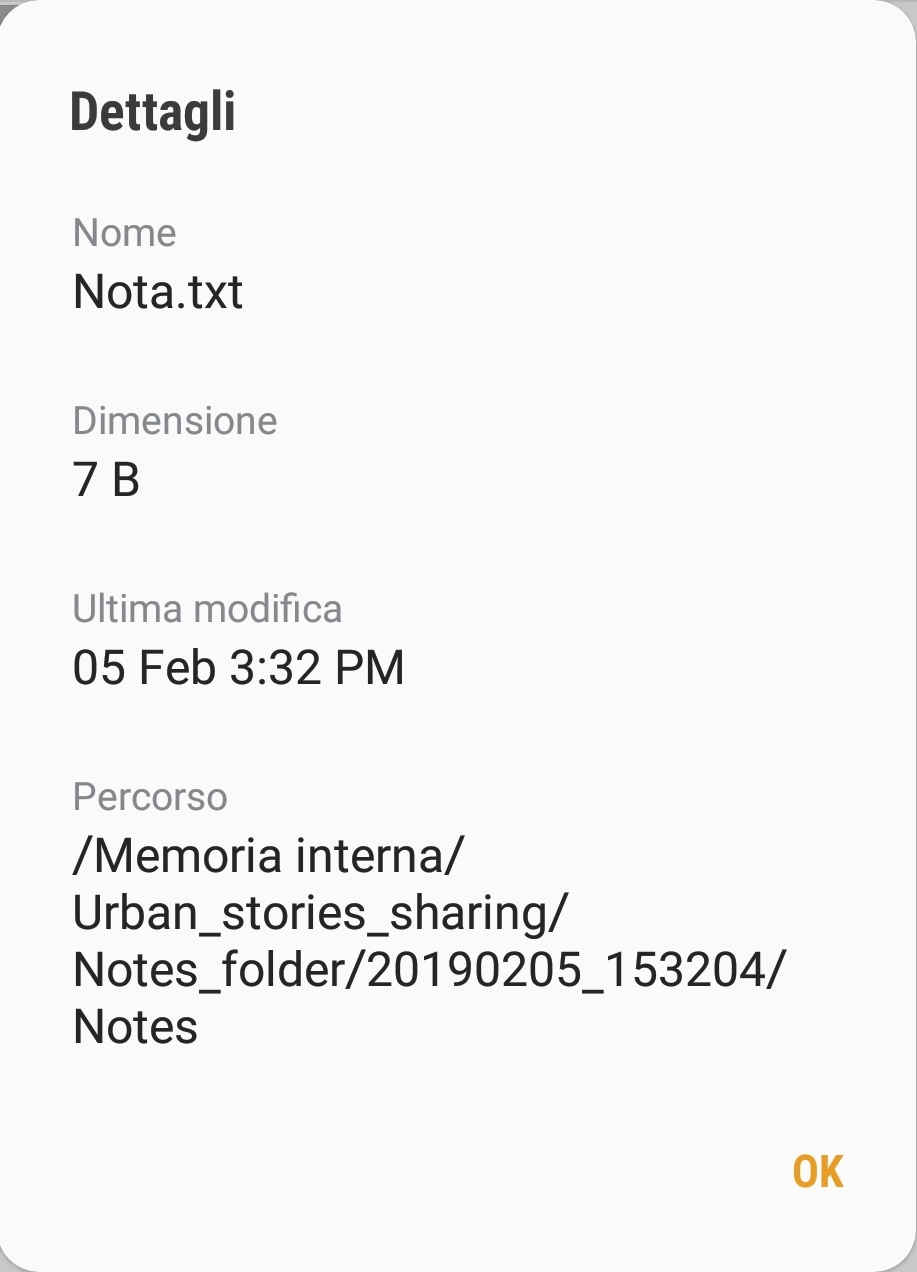
\includegraphics[scale=0.20]{Tesi/images/Percorso.jpg}
	\caption{\textit{Esempio di percorso per la nota scritta}}
	\label{percorso}
\end{figure}


\subsubsection{MySingleton.java}
Questa classe è stata creata per dare un appoggio per poter utilizzare la libreria Volley per permettere il caricamento sul repository centralizzato.
\subsubsection{GenericFileProvider.java}
Questa classe è stata creata estenendo la classe Provider, già implementata in Android, per poter salvare i file in locale.


\subsection{Layout}
\label{layout}
In informatica \textbf{XML} (sigla di eXtensible Markup Language) è un metalinguaggio per la definizione di linguaggi di markup, ovvero un linguaggio marcatore basato su un meccanismo sintattico che consente di definire e controllare il significato degli elementi contenuti in un documento o in un testo.\\
I layout dell'applicazione e le risorse utilizzate sono state implementate secondo questo metalinguaggio.\\
L'applicazione presenta \textbf{7 layout}:
\begin{itemize}
\item activity\_maps.xml
\item activity\_microphone.xml
\item activity\_modify\_photo.xml
\item activity\_modify\_video.xml
\item activity\_modify\_voice\_note.xml
\item activity\_post.xml
\item activity\_text\_note.xml
\end{itemize}
Nel capitolo \ref{chapter3} verranno mostrati nel dettaglio gli aspetti di questi layout.
\\In linea generale sono stati usati componenti di grandi dimensioni, molto evidenti ed i layout sono stati pensati per renderli più intuitivi e facili possibili, in vista del target di utenza scelto.

\subsection{Values}
\label{values}
Nella cartella values sono presenti le "risorse" a cui si affideranno i vari metodi e classi durante l'implementazione del progetto.
All'interno sono presenti:
\begin{itemize}
\item \textbf{colors.xml}\\
    In questo file possono essere definiti i vari colori che andranno poi ad essere utilizzati durante l'implementazione
\item \textbf{dimens.xml}\\
    All'interno possono essere definite alcune dimensioni che si andranno ad utilizzare durante l'implementazione
\item \textbf{strings.xml}\\
    All'interno saranno definite tutte le stringhe che verrano utilizzate durante l'implementazione dell'applicazione.
\item \textbf{styles.xml}\\
    In questo file, saranno definiti tutti gli stili che verranno utilizzati durante l'implementazione.
\end{itemize}
I values, sono molto utili, in quanto evitano l'hardcoding (soprattutto per quanto riguarda le stringhe).

\subsection{AndroidManifest.xml}
\label{manifest}
Ogni applicazione deve avere il file \textit{\textbf{AndroidManifest.xml}} (con questo preciso nome) alla radice del proprio progetto.
\\Il manifest, descrive le informazioni essenziali di ogni applicazione come: strumenti di Android, sistema operativo Android e Google Play.
\\Tra le altre cose, è richiesto il file manifest per dichiarare quanto segue:
\begin{itemize}
    \item \textbf{Nome del pacchetto dell'app}\\
    Quando si compila il codice, gli strumenti di compilazione sostituiscono questo valore con l'ID dell'applicazione dai file di build di Gradle, che viene utilizzato come identificatore di app univoco sul sistema e su Google Play. 
    \item \textbf{I componenti dell'app}\\
    Comprendono tutte le Activity, i servizi, i ricevitori di trasmissione e i fornitori di contenuti.\\
    Ogni componente può anche dichiarare funzionalità quali le configurazioni dei dispositivi che può gestire e filtri di intent che descrivono come il componente può essere avviato.
    
    \item \textbf{Autorizzazioni}\\
    Le autorizzazioni di cui l'app ha bisogno per accedere a parti protette del sistema o altre app.
\end{itemize}
Per poter utilizzare l'API di Google Maps bisogna però registrarsi sul sito web specifico ed ottenere una chiave univoca, senza la quale non sarebbe possibile visualizzare neanche la mappa.\\
Si può osservare l'implementazione all'interno del file \textbf{AndroidManifest.xml}:\\
\begin{lstlisting}
<meta-data
            android:name="com.google.android.geo.API_KEY"
            android:value="@string/google_maps_key" />
\end{lstlisting}
Dove \textit{\textbf{"@string/google\_maps\_key"}} è una stringa costante definita nella cartella \textit{\textbf{Values/strings.xml}} sopracitata e permetterà di accedere ai servizi delle mappe di Google.
\\\\Per quanto riguarda l'implementazione per il salvataggio dei file, attraverso il \textit{FileProvider.java} descritto nella sottosezione \ref{saving}, all'interno dell'Android Manifest, è stato così implementato:
\begin{lstlisting}
<provider
            android:name=".GenericFileProvider"
            android:authorities="com.example.android.fileprovider"
            android:exported="false"
            android:grantUriPermissions="true">
            <meta-data
                android:name="android.support.FILE_PROVIDER_PATHS"
                android:resource="@xml/provider_paths" />
        </provider>
\end{lstlisting}

\section{Design}
\label{design}
In questa sezione verranno presentati gli elementi principali di design di cui è composta l'applicazione.
\subsection{Material Button}
E' stata utilizzata una libreria che implementasse i Material Buttons, ovvero bottoni con cui l'utente potesse interagire, che seguissero le linee guida del Material Design.
\\La libreria in questione, è la seguente:
\textit{\textbf{android.support.design.button.Material Button}}
\\In Figura \ref{fig:MaterialButton} si può osservare un esempio di Material Button \textit{"Crea Nota"}:
\begin{figure}[!h]
    \centering
	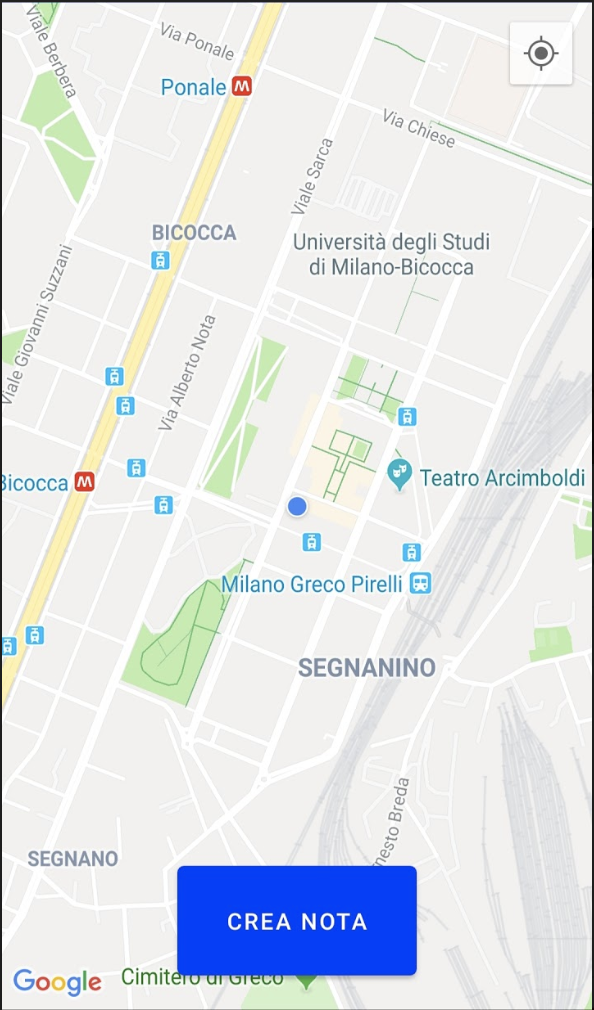
\includegraphics[scale=0.35]{Tesi/images/MaterialButton}
	\caption{\textit{Esempio di MaterialButton "Crea nota"}}
	\label{fig:MaterialButton}
\end{figure}

\subsection{Support Library Packages}
Una libreria, è un insieme di funzioni o strutture dati predefinite e predisposte per essere collegate ad un programma software attraverso un opportuno collegamento.
\\Lo scopo delle librerie software è fornire una collezione di entità di base pronte per l'uso, ovvero, riuso di codice, evitando al programmatore di dover riscrivere ogni volta le stesse funzioni o strutture dati e facilitando così le operazioni di sviluppo e manutenzione. Questa caratteristica si inserisce quindi nel più vasto contesto del "richiamo di codice" all'interno di programmi e applicazioni ed è presente in quasi tutti i linguaggi. 
\\I vantaggi principali derivanti dall'uso di un simile approccio sono i seguenti:
\begin{itemize}
    \item Si può separare la logica di programmazione di una certa applicazione da quella necessaria per la risoluzione di problemi specifici, quali il calcolo di funzioni matematiche o la gestione di collezioni
    \item Le entità definite in una certa libreria possono essere riutilizzate da più applicazioni
    \item Si può modificare la libreria separatamente dal programma, senza limiti alla potenziale vastità di funzioni e strutture dati man mano disponibili nel tempo
\end{itemize}
La libreria di supporto Android contiene diversi pacchetti di librerie che possono essere inclusi nell'applicazione. Ciascuna di queste librerie supporta una gamma specifica di versioni della piattaforma Android e un insieme di funzionalità.
\subsubsection{TextInput Layout}
Un'altra libreria utilizzata è stata la seguente: \textit{\textbf{android.support.design.widget.TextInputLayout}}
Ovvero è una libreria che permette l'utilizzo di Text Input, ovvero campi compilabili dall'utente, che permettono di seguire i canoni estetici e funzionali del Material Design.
\\In figura \ref{fig:textInput} se ne può osservare un esempio:
\\\begin{figure}[!h]
    \centering
	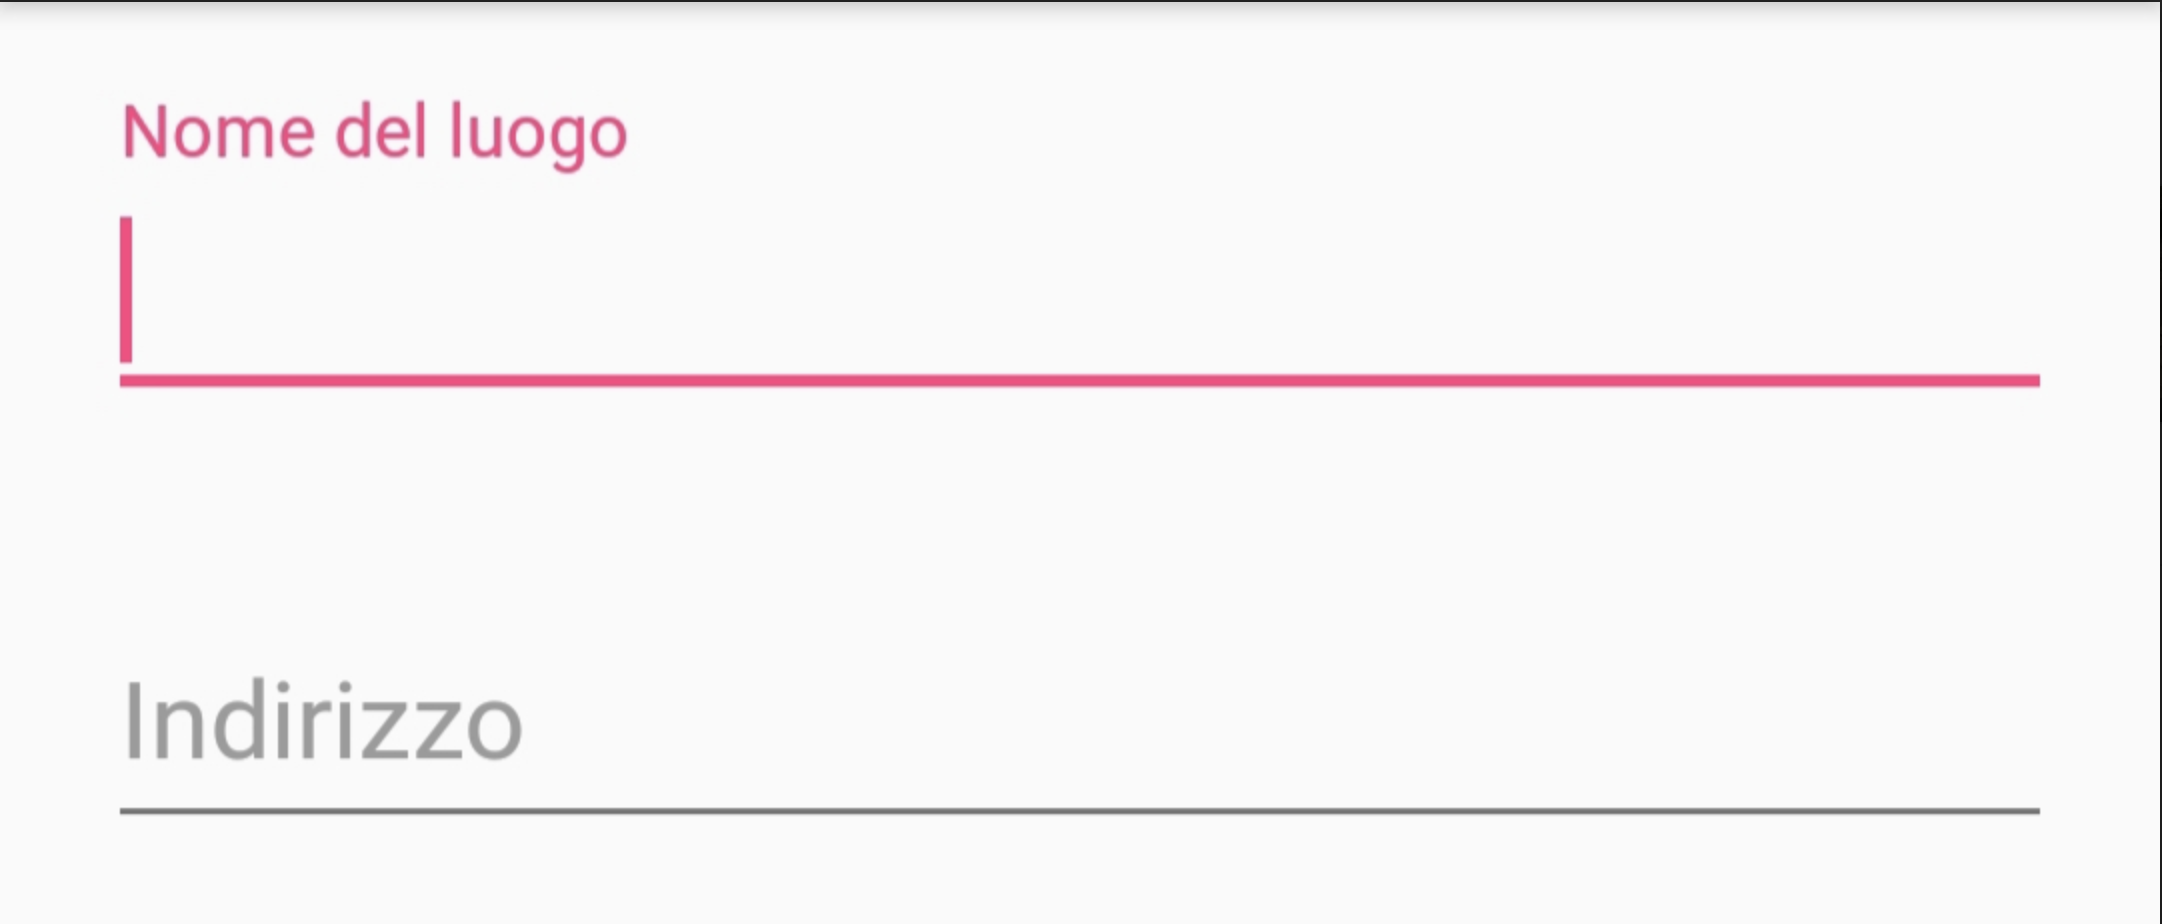
\includegraphics[scale=0.20]{Tesi/images/TextInput}
	\caption{\textit{Esempio di TextInput}}
	\label{fig:textInput}
\end{figure}
\subsubsection{Toolbar}
Ulteriore libreria utilizzata, necessaria al fine dello sviluppo, è stata la seguente: \textit{\textbf{android.support.v7.widget.Toolbar}}
Questa libreria ha fatto si che si potesse implementare una toolbar che permettesse all'utente di eseguire delle operazioni.
In figura \ref{fig:toolbar} si può osservare un esempio di toolbar:\\
\begin{figure}[!h]
    \centering
	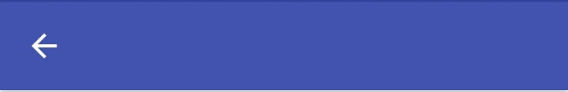
\includegraphics{Tesi/images/Toolbar}
	\caption{\textit{Esempio di Toolbar}}
	\label{fig:toolbar}
\end{figure}\\
\subsubsection{Card View}
Questa libreria utilizzata: 
\textit{\textbf{android.support.v7.widget.CardView}} ha permesso di aggiungere delle Card View, ovvero degli elementi che consentono di mostrare informazioni all'interno di schede che hanno un aspetto coerente su qualsiasi app. 
\\Queste schede sono utili per le implementazioni di Material Design e sono ampiamente utilizzate nei layout per le app TV.
In figura \ref{fig:cardview} si può nortare un esempio:
\begin{figure}[!h]
    \centering
	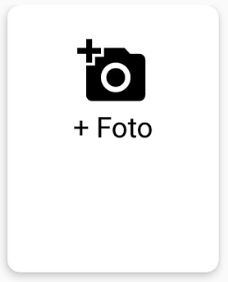
\includegraphics[scale=0.75]{Tesi/images/CardView}
	\caption{\textit{Esempio di CardView}}
	\label{fig:cardview}
\end{figure}
\subsubsection{Icone}
Tutte le icone utilizzate seguono le linee guida del Material Design e sono state implementate tramite Android Studio attraverso il Vector Asset, ovvero immagini vettoriali modificabili in fase implementativa.\\
Si può vedere un esempio di icone di Material Design in figura \ref{fig:icone}:
\begin{figure}[htp]
\centering

\includegraphics{Tesi/images/Video}\hfill
{
\includegraphics{Tesi/images/NotaScritta}}\hfill

\includegraphics{Tesi/images/Microfono}
\caption{\textit{Esempio icone Material Design}}\label{fig:icone}
\end{figure}\\

\section{Volley Library}
\label{volley}
Volley è una libreria HTTP che semplifica la connessione in rete per le app Android e, cosa più importante, più veloce. Volley è disponibile su GitHub.
\\Volley offre i seguenti vantaggi:
\begin{itemize}
    \item Pianificazione automatica delle richieste di rete.
    \item Più connessioni di rete simultanee.
    \item Supporto per la prioritizzazione delle richieste.
    \item API di richiesta di cancellazione. È possibile annullare una singola richiesta oppure è possibile impostare blocchi di richieste da annullare.
    \item Facilità di personalizzazione
    \item Strumenti di debug e tracciamento.
\end{itemize}
All'interno di questo progetto di stage, è stata utilizzata questa libreria per eseguire la richiesta \textbf{POST}, ovvero, la richiesta HTTP per inviare i file multimediali al repository centralizzato \cite{volley}.

